%-----------------------------------------------------
% Chapter 3: Descripción del prototipo
%-----------------------------------------------------
\chapter{Desarrollo}
\label{chap: cap3}

\section{Descripción general del prototipo}
El prototipo de entorno colaborativo cuenta con una arquitectura que permite desplegar un aplicación multiplataforma accesible a través de un navegador web.

Está conformado por 2 componentes de software.
El primer componente se denomina Capa de Servicios (Backend) y es una aplicación de servidor que permite:
\begin{itemize}
  \item Iniciar y parar los servicios. 
  \item Conocer el estado de los servicios.
  \item Guardar registros de bitácora (LOGS).
  \item Gestionar peticiones de los clientes.
  \item Exponer la interfaz de usuario (Segundo componente).
\end{itemize}

El segundo componente es una interfaz construida con tecnologías web (Front-End) y se ejecuta en un navegador web convencional, permitiendo al usuario:
\begin{itemize}
  \item Visualizar un modelo 3D con funciones de acercamiento (zoom), rotación y translación.
  \item Compartir el entorno colaborativo mediante un hiperenlace web.
  \item Visualizar y Manipular parámetros relacionados al modelo 3D de manera sencilla e intuitiva.
  \item Agregar información extra (anotaciones, imágenes, etc) relacionados al modelo.
  \item Generar nuevas versiones de los modelos en un mismo espacio de trabajo.
  \item Explorar todas las versiones y los cambios de parámetros respecto a su antecesor.
  \item Recibir notificaciones referente a las acciones de otros usuarios sobre el entorno.
 
\end{itemize}

\section{Enfoque Lean UX}

Lean UX \cite{Gothelf2013} es el enfoque o metodología que acompaña la construcción del prototipo de este trabajo final, a continuación se explican los conceptos que motivan la elección de esta metodología.


\begin{figure}
\centering
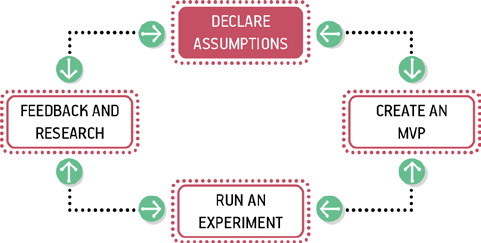
\includegraphics[width=9cm]{Img/UX/UX-0.png}
\caption[(optional short caption)]{\label{us_figure} Enfique LEAN UX}
\end{figure}

Desde 1980 hasta fines de 1990 los diseñadores se enfocaron en el diseño de software de la misma manera que lo habían hecho con el resto de materiales. Cuando se diseña para producir algo físico, se necesita tener muy claro lo que se hace antes de iniciar la producción física, porque la producción es costosa. Es costoso poner en marcha una fábrica para producir bienes físicos. En el trabajo con software, los diseñadores tuvieron que enfrentar nuevos retos, descubrir los nuevos medios y, a medida que lo hacían, aparecían nuevas especialidades, como el diseño de interacción o la arquitectura de información. Sin embargo, en esa época la práctica de los diseñadores apenas cambió. Todavía diseñaban los productos de manera tradicional, con mucho detalle y por adelantado, porque había un proceso de "fabricación": había que hacer copias de los trabajo en discos flexibles y CDs y distribuirlas de la misma manera en la que se distribuyen los bienes físicos. Todavía era muy costoso cometer errores.\vskip En la actualidad internet ha cambiado la distribución de software de una manera radical. La mayoría del software se distribuye en línea y al desaparecer el proceso físico de fabricación se puede trabajar con ciclos de producción mucho más cortos.
Los equipos de desarrollo de software utilizan técnicas como el desarrollo ágil, la integración continua y el despliegue continuo reduciendo drásticamente el tiempo para generar nuevas cambios en el software. Estos equipos suben código a producción en el tiempo que tardaríamos en guardar cualquier archivo en una computadora. Además, utilizan esos ciclos cortos como ventaja competitiva, producen nuevas versiones del software tiempos acotados, lo que les permite obtener retroalimentación del mercado e iterar incorporando lo que han aprendido y tal vez sin advertirlo aumentan las expectativas de los clientes que pueden obtener más calidad en menos tiempo. La verdad es que, en este nuevo contexto, las prácticas de pensar todo al inicio de los procesos ya no funcionan. \vskip
\textit{Lean User Experience} (Lean UX) se puede traducir como \textit{Experiencia de Usuario limpia o sin desperdicios} y se describe como una nueva etapa evolutiva en el diseño de productos. El objetivo es tomar las mejores herramientas del diseño y adaptarlas a esta nueva realidad.
Lean UX\cite{Nyamsuren2015} es profundamente colaborativo, porque los diseñadores no están aislados del resto del equipo de trabajo ya que permite implementar técnicas para construir una comprensión compartida, se puede tener retroalimentación con los usuarios finales y  replantear las conversaciones de diseño en términos objetivos, obtener métricas sobre las funcionalidades, analizar y ajustar.
Otra ventaja importante es cambiar la forma en que se comunica el diseño del producto, en lugar de comunicar características y documentos exhaustivos se puede comunicar funcionalidad.


3 pilares principales de Lean UX:\vskip
\textbf{1. Design Thinking o Pensamiento de Diseño:} Alienta al equipo a colaborar en todas las etapas del proyecto y a considerar el producto desde una perspectiva global, utilizando la sensibilidad y los métodos de los diseñadores para satisfacer las necesidades del usuario final con soluciones tecnológicamente viables.

\textbf{2. Desarrollo Ágil}:
 Aplica los cuatro principios básicos del desarrollo Ágil al diseño de los productos.

\begin{itemize}
\item
\textbf{Los individuos y las interacciones son más importantes que los procesos y las herramientas}\vskip
Para generar rápidamente las mejores soluciones, es necesario implicar al todo el equipo. El intercambio de ideas deberá ser libre y frecuente. La conversación fluida entre colegas deberá primar por encima de las restricciones propias de las herramientas, ya sea en los procesos o en la producción.
\item
\textbf{El software funcional es más importante que la documentación exhaustiva}\vskip
Se pueden encontrar múltiples soluciones para todos los problemas de negocio y todos los miembros del equipo podrán tener una opinión diferente de cuál es la mejor. El reto está en averiguar cuál de ellas es la que tiene más posibilidades. Por eso, cuanto antes se cuente con un software que funcione, antes se puede encontrar la solución que mejor se adapte a los requerimientos.
\item
\textbf{La colaboración con los clientes es más importante que la negociación de contratos con ellos}\vskip
Si el equipo colabora con los usuarios/clientes, hay un entendimiento común sobre los problemas y las posibles soluciones. Cualquier decisión que se adopte después se tomará por consenso, lo que se traduce en iteraciones más rápidas y una verdadera implicación de todos los actores con la ventaja de trabajar siempre con soluciones validadas. Además, como todos los miembros del equipo participan en la toma de decisiones, no se requieren tantas entregas de documentación por escrito.
\item
\textbf{La respuesta a los cambios es más importante que la planificación}\vskip
Lean UX asume que los diseñadores del producto inicial no encontrarán la solución a la primera, por lo que el objetivo consiste en averiguar qué han hecho mal lo antes posible. Una vez que se descubra lo que funciona y lo que no, se pueden ajustar las propuestas y volver a probarlas. Así, la retroalimentación mantendrá ágil al equipo, dirigiendo la solución siempre en la dirección correcta.
\end{itemize}

\textbf{3. Método Lean Startup}: Utiliza un bucle de retroalimentación llamado  "\ Construir-Medir-Aprender" para minimizar el riesgo del proyecto, haciendo que los equipos construyan y aprendan rápidamente.
Los equipos construyen productos viables mínimos del inglés \textit{Minimum Viable Product} (MVP) y los envían para comenzar el proceso de aprendizaje tan pronto como sea posible.\vskip
Lean Startup\footnote{\ https://es.wikipedia.org/wiki/Lean_startup}  desde el principio aboga por la creación de prototipos rápidos para comprobar, por un lado, que las suposiciones son correctas y, por otro, para conseguir retroalimentación de los clientes de forma inmediata y así poder mejorar el software más rápido que las prácticas tradicionales de ingeniería de software.\vskip
Lean UX, por su parte, es una implementación directa de esta filosofía aplicada al diseño de productos. Cada diseño es una solución propuesta, una hipótesis. Su objetivo consiste en validar la solución de la manera más eficiente posible mediante la realimentación. La cosa más pequeña que se puede construir para probar cada hipótesis es el Producto Viable Mínimo  MVP. 
Lean UX funciona como una práctica para entender rápidamente la función de un producto. Para ello elije un camino colaborativo y multidisciplinario; reduce el énfasis por la documentación exhaustiva y aumenta el enfoque en la construcción de un entendimiento compartido del producto que está siendo diseñado.

Por todo lo señalado se considera que este enfoque es el adecuado para abordar el trabajo en la aplicación COCADA, como consecuencia se obtiene: un equipo que trabaja de forma colaborativa, iterativamente y en paralelo, que reduce al mínimo los documentos entregables y que se centra en el software funcional y en la retroalimentación con el usuario final.


\section{Visión, marco y resultados}

Los proyectos de diseño de experiencia de usuario (UX) han estado enmarcados, tradicionalmente, por los requerimientos y las entregas. A los equipos se les suministraban requerimientos para que produjeran entregas. Lean UX cambia por completo este marco de trabajo. El objetivo no es generar un documento entregable, sino producir un resultado. \textbf{No se comienza con requerimientos, sino con suposiciones}. A partir de ellas, se crean y prueban hipótesis. Entonces se puede medir si gracias a las hipótesis se ha conseguido alcanzar los resultados buscados. La herramienta principal de este nuevo enfoque del trabajo son \textbf{las declaraciones de hipótesis}. Estas declaraciones son el punto de inicio de los proyectos. Establecen una visión clara del trabajo y consiguen algo importante: que los miembros del equipo de desarrollo y los gestores del proyecto dejen de hablar sobre la salida que se espera, por ejemplo, \textit{"Vamos a crear una función para visualizar modelos 3d paramétricos"} y comiencen a hacerlo sobre los resultados del proyecto, por ejemplo, \textit{"Queremos aumentar el número de comparticiones de diseños entre los actores"}.\vskip
Para obtener las suposiciones se tiene que hacer una investigación previa

Una declaración de hipótesis es una manera de expresar las suposiciones que tenemos de nuestro proyecto de una forma comprobable. Está compuesta de los siguientes elementos:

\subsection{Declaración de suposiciones}

Las suposiciones son una declaración de alto nivel que pensamos que es cierta.

Todos los proyectos, no solo los de esta metodología, comienzan de este modo pero, normalmente, no hacen explícitas sus suposiciones. En lugar de ello, se ignoran o, en el peor de los casos, se tratan como si fueran hechos probados.

\textbf{Quiénes}: La declaración de suposiciones es un ejercicio de grupo. Se reúne al todo el equipo, asegurándose de que todas las disciplinas estén representadas, se incluye en él a todos los que puedan saber cosas importantes para el proyecto. Por ejemplo, si el proyecto trata de solucionar una queja habitual por parte de los clientes, podría ser beneficioso que se incluyera a algún representante del servicio al cliente en el servicio de call center. Los encargados de ese servicio hablan más con los clientes que nadie de la empresa, por lo que seguramente sabrán más sobre este tema que el resto del equipo.


\textbf{Preparación}: Es necesario que, antes de empezar, el equipo sepa el problema con el que se trabajará para que puedan preparar el material que necesiten. En la preparación se debe recurrir a técnicas de investigación para recolectar información sobre los usuarios y sus necesidades, en la Fig. 3.2 se puede observar un diagrama de decisión de las técnicas utilizadas para este trabajo.

\begin{figure}
\centering
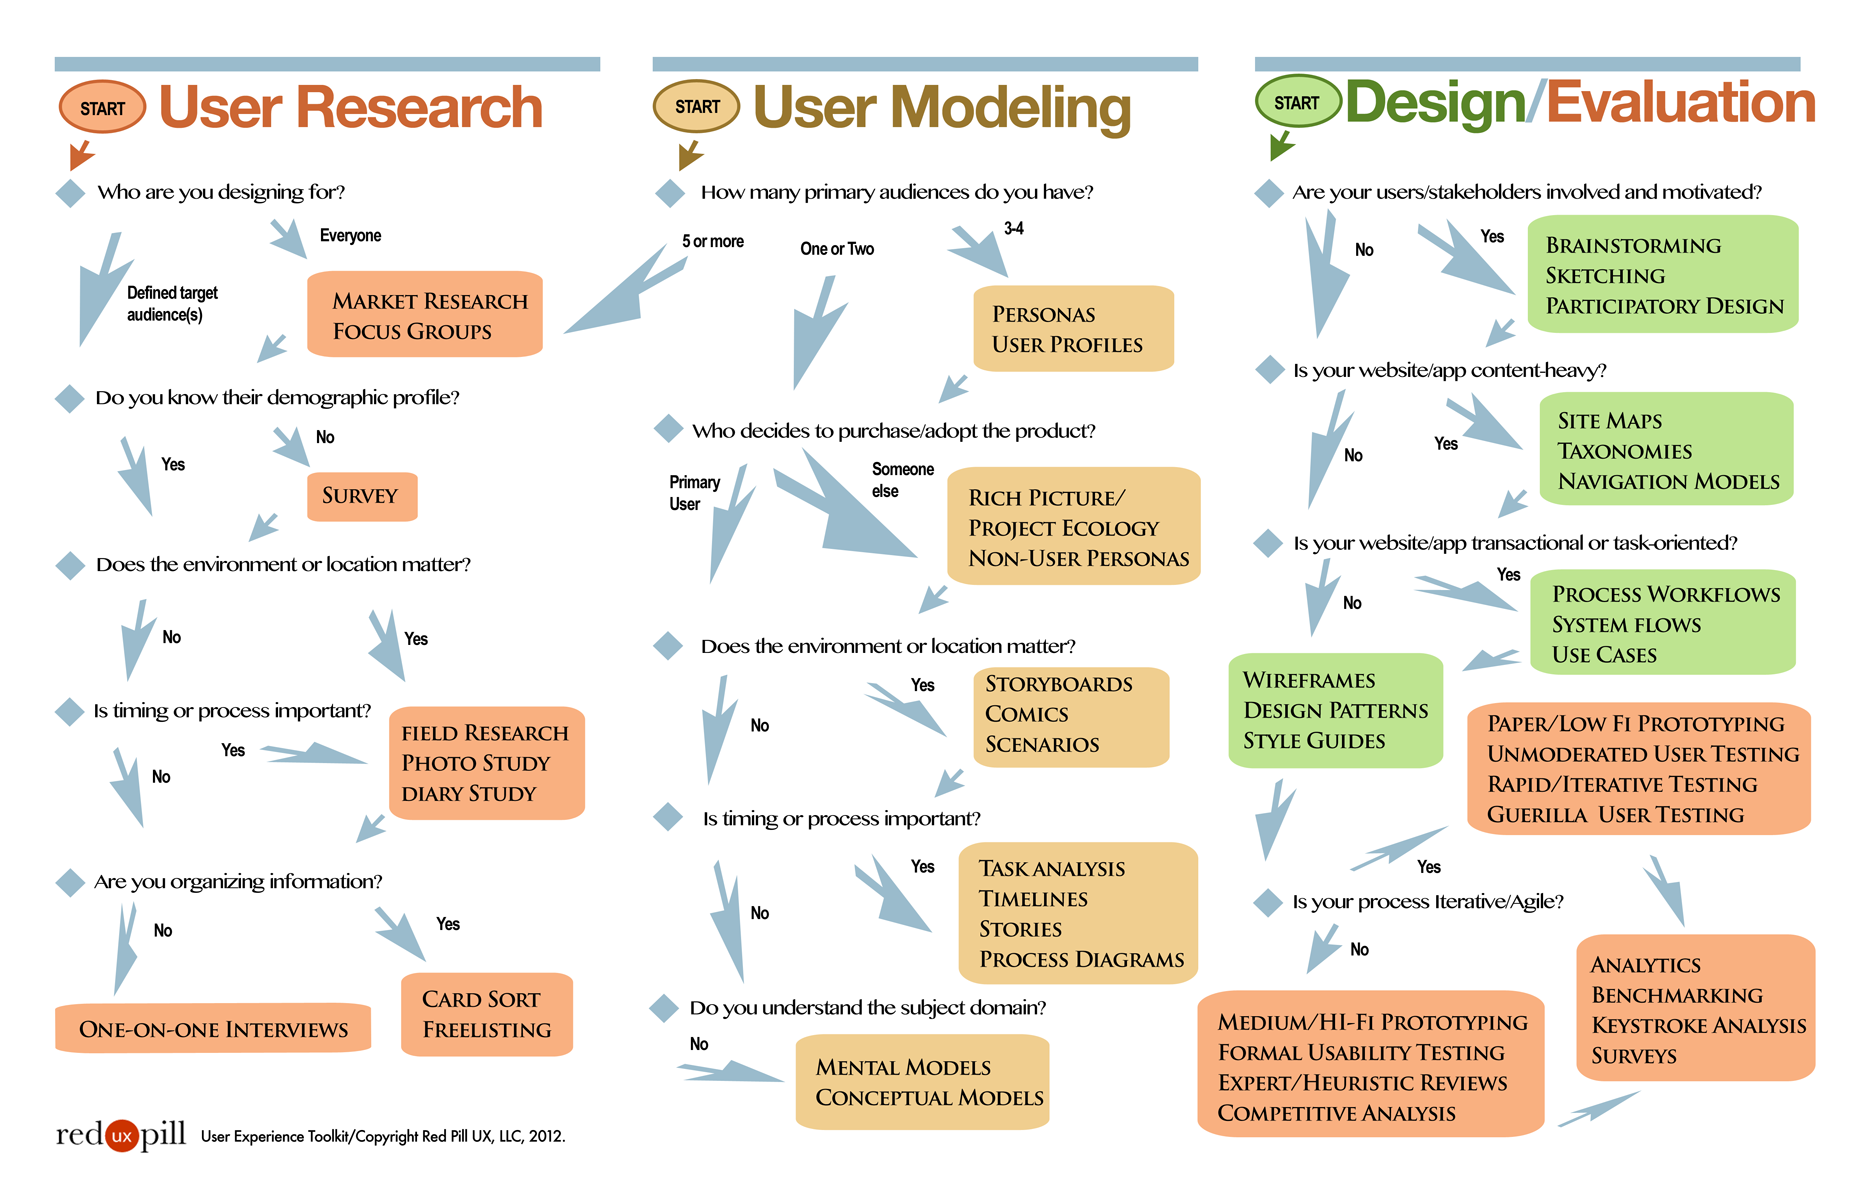
\includegraphics[width=16cm]{Img/CPD/3-FLOW.png}
\caption[Diagrama de desición de investigación del usuario]{\label{us_figure} Diagrama de desición de investigación del usuario}
\end{figure}




\subsection{Hipótesis}
Descripción general de lo que se debe hacer

Desarrollar un software de comunicación eficiente en la revisión de diseños para un equipo multidisciplinario
logrará una mayor tasa de participación y un aumento en la satisfacción de los involucrados.
Se verificará que esto es cierto cuando aumenten las opiniones de los involucrados y se pueda registrar la evolución del diseño.


\subsection{Proto-personas}

Se usan Modelos de personas como arquetipos de usuarios que a su vez comparten  características de determinados grupos de clientes o usuarios.
En Lean UX, se invierte el orden de operaciones en el proceso persona, se comienza con suposiciones y luego se hace una investigación para validar las suposiciones. En lugar de pasar meses en el campo entrevistando a la gente, se invierten horas creando proto-personas o simplificaciones de personas para generar la conjetura más aproximada de quién está utilizando (o va a utilizar) el software y por qué. 

Ver fig 3.2 y 3.3

\begin{figure}
\centering
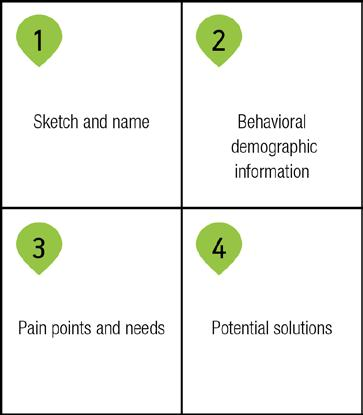
\includegraphics[width=9cm]{Img/UX/proto-table.jpg}
\caption[Proto-persona (optional short caption)]{\label{us_figure} Tabla de proto-persona}
\end{figure}

\begin{figure}
\centering
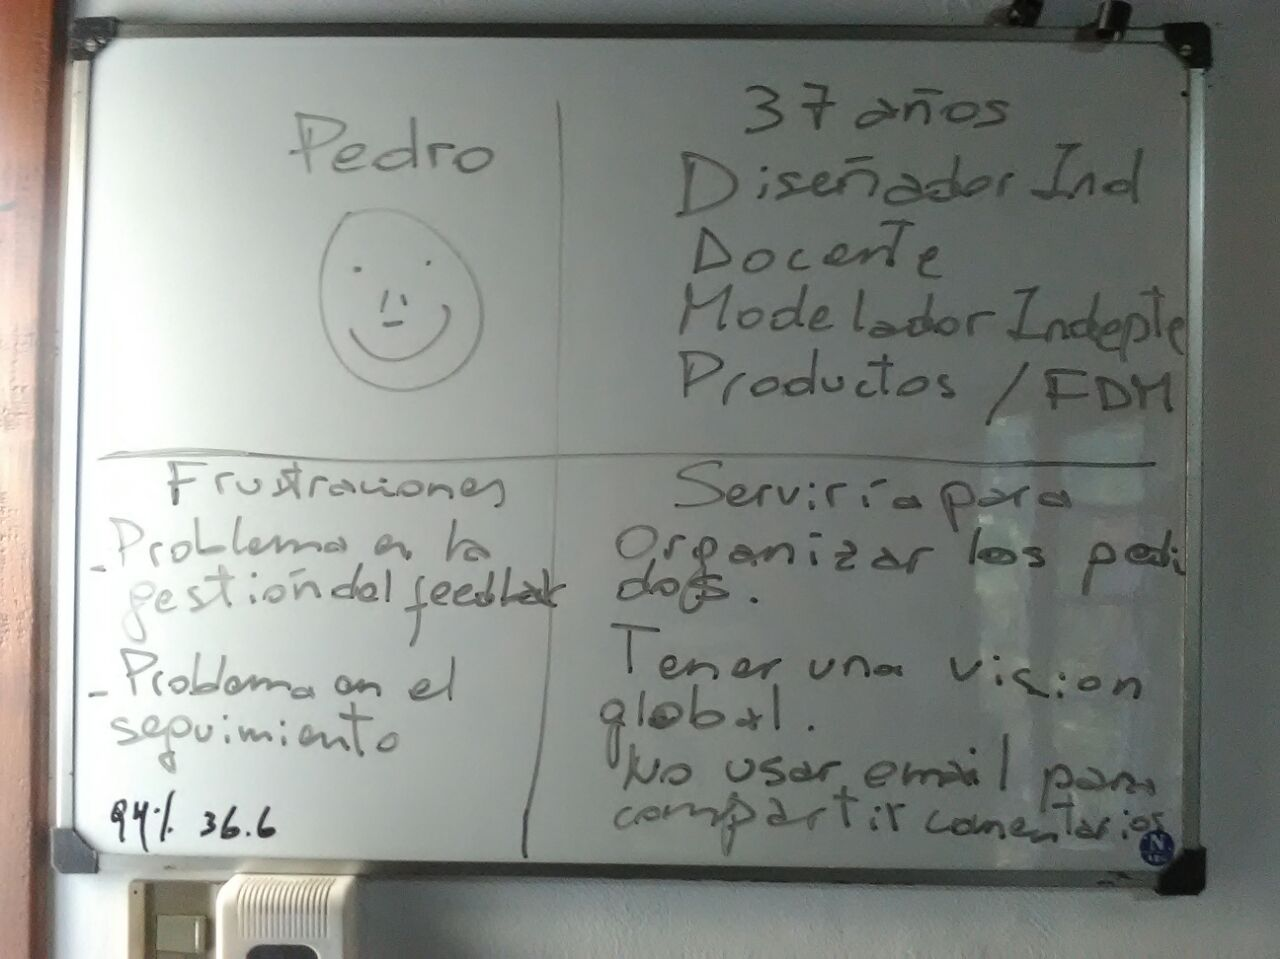
\includegraphics[width=9cm]{Img/UX/UX-proto.jpg}
\caption[Proto-persona (optional short caption)]{\label{us_figure} Proto-persona}
\end{figure}

\subsection{Características}
 Una vez que se obtiene una lista de los resultados buscados por los usuarios y se han establecido los diferentes grupos, es hora de empezar a pensar en qué tácticas, características, productos y los servicios que se pueden proponer para alcanzar esos resultados deseados. El proceso de diseño comienza cuando se tiene noción de alguna característica y se trabaja para justificar la característica. En Lean UX, las características existen exclusivamente para satisfacer las necesidades del usuario.

\subsection{Sub-hipótesis con funcionalidades: Historias}

Tabla:

Se necesita hacer / Para qué persona / Qué soluciona.

Se necesita desarrollar un visualizador de modelos 3D / Para la persona con rol diseñador experto (XXX) / que solucione la visualización online de los avances de su trabajo.



\section{Diseño colaborativo}

\subsection{Mockup}

\subsection{Guías de estilo: Bulma}


\begin{figure}
\centering
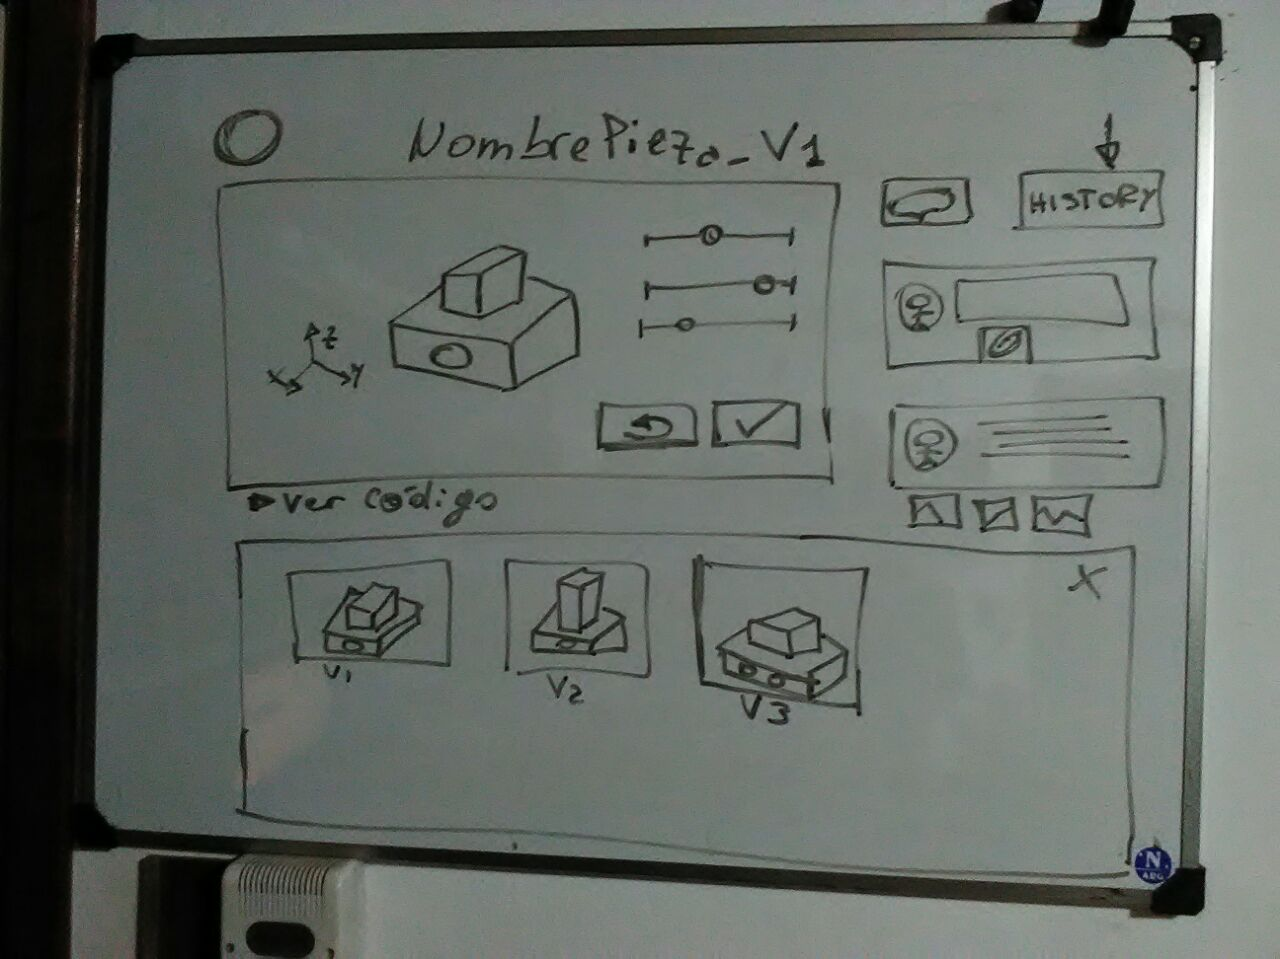
\includegraphics[width=9cm]{Img/UX/UX-proto1.jpg}
\caption[Proto-persona (optional short caption)]{\label{us_figure} Mockup}
\end{figure}

\section{MVP - Prototipado}
\subsection{Prototipado rápido HTML más Bulma}

\begin{figure}
\centering
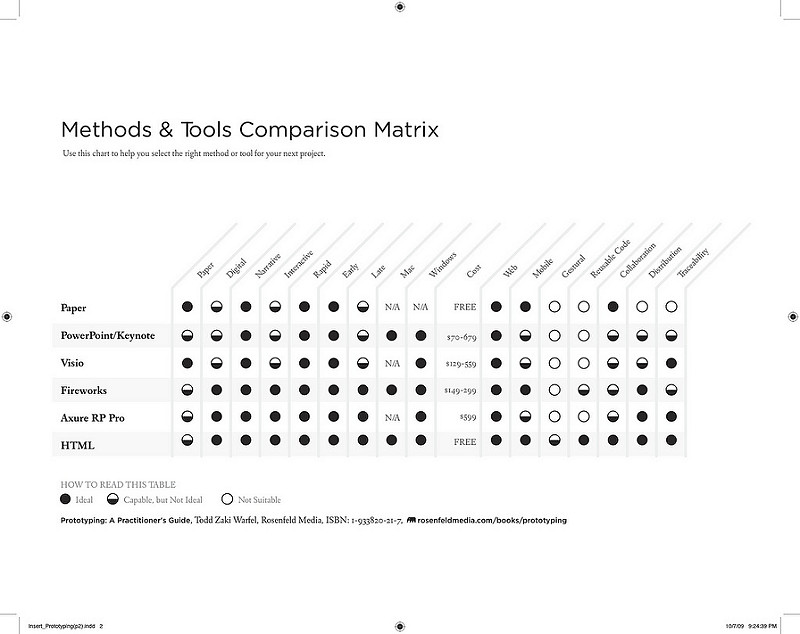
\includegraphics[width=16cm]{Img/UX/UX-matrix.jpg}
\caption[Proto-persona (optional short caption)]{\label{us_figure} Matriz de herramientas para prototipado. Extender a nuevas herramientas}
\end{figure}

\section{Herramientas tecnológicas para el desarrollo}

\subsection{Lenguaje Ubicuo: De Historias a Escenarios y tests}

Scenario: Listar los Trabajos\vskip0mm
  Given: Estoy en URL\vskip0mm
  Then: Veo el título "Pieza de Pruebas"\vskip10mm
 
Scenario: Acceder al Escritorio de Trabajo\vskip0mm
  Given: Estoy en URL\vskip0mm
  When: Hago click en "Pieza de Pruebas"\vskip0mm
  Then: Estoy en URL\vskip0mm
  Then: Veo el título "Pieza de Pruebas"\vskip0mm
  And: Veo la etiqueta "Alto"\vskip0mm
  And: Veo la etiqueta "Ancho"\vskip0mm
  And: Veo la etiqueta "Profundidad"\vskip0mm
  And: Veo el Visor de la Pieza "stl-view"
  
\subsection{Especificación BDD Escenarios, Cucumber, etc}

\subsection{Programación SPA (Single Page App)}

\begin{displayquote}
An SPA is an application delivered to the browser that doesn’t reload the page during use. Like all applications, it’s intended to help the user complete a task, such as “write a document” or “administer a web server.” We can think of an SPA as a fat client that’s loaded from a web server. \cite{Mikowski2015}
\end{displayquote}

\say{The single-page web interface is composed of individual components which can be updated/replaced independently, so that the entire page does not need to be reloaded on each user action.\cite{Mesbah2007}}


\subsection{Visualización y datos (WebGL, OpenJSCAD)}

\subsection{Frontend Vue.js}

\subsection{Backend (Node.js, Express, GraphQL, ES 2015 )}


\section{Métricas, ecuaciones, fórmulas, posibilidades}


\section{Construcción del sistema}

\subsection{Modelado de Classes}

\subsection{Diseño y Código en JS (FLUX?)}

\subsection{API: GraphQL}


\section{Funcionalidades}

\subsection{Control de versiones}

\subsection{Integración con otras plataformas (embed)}

\subsection{Compartir proyectos (share)}

\subsection{Exportar modelos}

\subsection{Extras: Anotaciones, comentarios, adjuntar imagen, chat, etc}
